% Group 7 Data Mining final report draft. Compile twice with XeLaTeX.
% Official acmart class (sigconf, nonacm); all figures are native to this file.
\documentclass[sigconf,nonacm,10pt,balance=false]{acmart}
\settopmatter{printacmref=false,printccs=false,printfolios=true}
\raggedbottom
\emergencystretch=1.7em
\tolerance=1400
\hyphenpenalty=650
\hyphenation{as-sis-tant in-de-pen-dent in-de-pen-dent-ly ex-act im-prove-ment ac-cu-ra-cy re-triev-al}
\pagestyle{plain}
\usepackage{fontspec}
\newfontfamily\vietfont{DejaVu Serif}
\DeclareRobustCommand{\vn}[1]{{\vietfont #1}}
\usepackage{array,tabularx,tikz}
\usetikzlibrary{arrows.meta,positioning}
\definecolor{inkblue}{HTML}{163B55}
\definecolor{softblue}{HTML}{EAF2F7}
\definecolor{tealchart}{HTML}{267E7B}
\definecolor{rustchart}{HTML}{A65C38}
\hypersetup{colorlinks=true,urlcolor=inkblue,linkcolor=inkblue}
\pdfstringdefDisableCommands{\def\vn#1{#1}\def\quad{, }\def\enspace{, }}
\newcommand{\baseurl}{https://github.com/xphiwork-dot/mpr-study/blob/main}
\newcommand{\repo}[2]{\href{\baseurl/#1}{#2}}
\newcommand{\paper}[2]{\href{https://arxiv.org/html/2508.13250v1\##1}{#2}}
\newcommand{\emphlabel}[1]{\par\smallskip\noindent\textbf{#1}\enspace}
\newcommand{\smallcaption}[2]{\par\smallskip\noindent{\small\textbf{#1.} #2}\par\smallskip}
\newcommand{\localtable}{\small\setlength{\tabcolsep}{3pt}\renewcommand{\arraystretch}{1.15}}
\newcommand{\cbox}[1]{\colorbox{softblue}{\parbox{\dimexpr\columnwidth-2\fboxsep\relax}{\small #1}}}
\title[Memory for Multi-Hop Personalized Reasoning]{Explicit vs. Implicit Memory for Multi-Hop Personalized Reasoning: A Critical Reproduction}
\subtitle{Data Mining Final Project Report | Group 7 | Advisor: \vn{Nguyễn Võ Lê Duy}}
\author{\mbox{\vn{Nguyễn Xuân Phi}}\enspace\mbox{\vn{Lê Hải Phong}}\enspace\mbox{\vn{Trần Nguyên Phong}}\enspace\mbox{\vn{Phan Văn Phú}}}
\renewcommand{\shortauthors}{Group 7}
\begin{document}
\begin{abstract}
Multi-hop personalized reasoning requires connecting several user facts that may not resemble the original query. We summarize Zhang et al.'s benchmark and HybridMem method and test selected claims on a smaller compute budget. On 306 matched questions, sequential and multi-path reasoning outperform one-call retrieval-augmented generation. Multi-path reasoning shows no detectable edge over five-step sequential reasoning despite using 12 instead of five calls. With gold evidence fixed, five-step reasoning improves exact match by 25.8 percentage points; retrieval alone cannot explain the gain. Larger retrieval sets improve evidence recall without a detectable gain in answer accuracy. We also audit numeric overlap and examine a small HybridMem probe.
\end{abstract}
\maketitle
\section{Introduction}
Personalized assistants can often answer simple questions by locating one statement. A multi-hop question is different: the first relevant statement may contain the name needed to retrieve the second, and the final fact may share no distinctive terms with the original query. The assistant must find evidence as its understanding of the question changes, then combine that evidence correctly.

Zhang et al.\ compare memory stored outside the model against memory learned in its parameters. Their benchmark allows both the evidence store and the reasoning procedure to vary. Our goal is not to match their absolute scores. We ask which comparisons remain visible on smaller hardware, what additional calls buy, and which explanations are supported by the evidence.

For example, answering where Alice's husband works requires identifying Bob, linking him to David's department, and locating that department in New York. Alice's own workplace in Boston is a plausible search result but answers the wrong question. The key retrieval problem is that David is absent from the initial query.

\newpage
\section{Problem Setup and MPR Dataset}
Let $\mathcal S=\{s_1,\ldots,s_n\}$ be a collection of single-hop user statements. Given a question $q$, the model predicts $\hat a=f(q;\mathcal S)$. The task requires a set of user facts that jointly supports the gold answer $a$, while no one statement suffices. General knowledge can assist with an operation such as date comparison, but cannot substitute for the user-specific facts.

\subsection{From graph edges to test questions}
The authors instantiate a meta-graph into 12 synthetic user graphs. The blueprint specifies 108 entity types and 34 relation types. Entity and attribute edges become natural-language statements; value relations permit general operations such as comparing two quantities. The authors sample paths of 2--10 hops, add distinguishing information when a matched attribute is ambiguous, and rewrite each path as a question. The endpoint provides the answer, and the original path and supporting statements provide evidence annotations.

\begin{center}
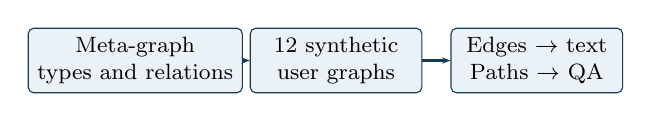
\begin{tikzpicture}[x=1cm,y=1cm, every node/.style={font=\footnotesize, align=center}, box/.style={draw=inkblue,fill=softblue,rounded corners=2pt,minimum width=2.18cm,minimum height=.82cm}]
\node[box] (a) at (0,0) {Meta-graph\\types and relations};
\node[box] (b) at (2.55,0) {12 synthetic\\user graphs};
\node[box] (c) at (5.10,0) {Edges $\to$ text\\Paths $\to$ QA};
\draw[-{Stealth[length=3pt]},inkblue,thick] (a)--(b);
\draw[-{Stealth[length=3pt]},inkblue,thick] (b)--(c);
\end{tikzpicture}
\end{center}
\smallcaption{Figure 1}{Benchmark generation. Redrawn from Zhang et al., \paper{S3.SS3}{\S3.3 and Fig.~2(a)}. Each test item retains the question, answer and evidence path.}

\emphlabel{Scale and coverage.} Paper Table 2 reports 157,166 statements and 108,000 questions (about 13,100 statements per user). Our release audit covers 32,399 questions; the published design and audited release are distinct counts.

\emphlabel{Evaluation.} The system can prepare memory from the user's statements, but at test time receives only the question. The gold evidence stays hidden except under the Oracle control. The paper compares normalized answers by exact match (EM). This scores the final answer, not whether the model followed the intended path. Evidence recall can diagnose a failure to retrieve facts, but high recall does not establish correct reasoning.



\clearpage
\section{Methodology and Proposed HybridMem}
\subsection{Memory and reasoning are separate choices}
\emphlabel{Explicit memory.} The model receives retrieved statements as text. SparseRAG uses BM25s term matching, DenseRAG uses E5 embeddings, TreeRAG searches a hierarchy of summaries, and GraphRAG uses extracted entities and relations. The paper usually returns $k=20$ statements. The no-memory control (Ignoramus) sees none; Oracle sees the gold statements and thus removes evidence retrieval errors without guaranteeing a correct answer.

\emphlabel{Implicit memory.} Low-rank adaptation (LoRA) changes the model parameters instead of passing user statements in the prompt. MaskSFT trains the model to restore masked facts. AskSFT rewrites facts as question--answer pairs. In both closed-book settings, the model must recall the facts and compose them at test time.

\emphlabel{Reasoning structures.} Naive reasoning (NR) answers in one call. Sequential reasoning (SR) extends one chain; under RAG, the evolving state can guide repeated retrieval. Multi-path reasoning (MR) considers multiple continuations and chooses a path to extend. Decomposition reasoning (DR) divides the question into subquestions, solves them, and merges the intermediate answers. DR has to choose what to ask before it has discovered the bridge entities, which can make an initial mistake hard to recover from. Conversely, sequential reasoning can also carry a wrong intermediate result forward.

\subsection{HybridMem: evidence also selects an adapter}
HybridMem keeps explicit evidence but does not commit to a single globally fine-tuned adapter. Offline, the method embeds each statement, groups statements into local clusters via $k$-means, and trains a separate LoRA adapter on each cluster while building a retrieval index. Online, retrieved statements vote by cluster label; the winning label selects the adapter. The model then uses that adapter together with explicit evidence.

Local adapters may avoid forcing unrelated facts into a single update. But a reasoning chain can span clusters, and poor retrieval can steer the vote toward the wrong adapter. The paper measures the combined method; it does not isolate the effects of clustering and routing.

\newpage
\begin{center}
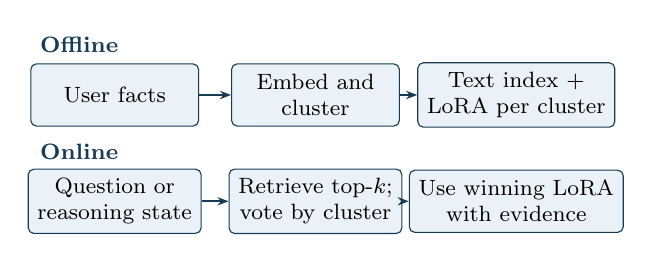
\begin{tikzpicture}[x=1cm,y=1cm,every node/.style={font=\footnotesize,align=center},box/.style={draw=inkblue,fill=softblue,rounded corners=2pt,minimum width=2.13cm,minimum height=.79cm}]
\node[anchor=west,font=\footnotesize\bfseries,text=inkblue] at (-1.07,.64) {Offline};
\node[box] (a) at (0,0) {User facts};
\node[box] (b) at (2.55,0) {Embed and\\cluster};
\node[box] (c) at (5.10,0) {Text index +\\LoRA per cluster};
\node[anchor=west,font=\footnotesize\bfseries,text=inkblue] at (-1.07,-.72) {Online};
\node[box] (d) at (0,-1.35) {Question or\\reasoning state};
\node[box] (e) at (2.55,-1.35) {Retrieve top-$k$;\\vote by cluster};
\node[box] (f) at (5.10,-1.35) {Use winning LoRA\\with evidence};
\foreach \x/\y in {a/b,b/c,d/e,e/f} \draw[-{Stealth[length=4pt]},thick,inkblue] (\x)--(\y);
\end{tikzpicture}
\end{center}
\smallcaption{Figure 2}{HybridMem, redrawn from Zhang et al., \paper{S6.SS2}{\S6.2}. Retrieved facts serve two purposes: supply context and route inference to an adapter.}

\section{Experiments and Group Reproduction}
\subsection{What the paper reports}
The main paper experiments use Qwen2.5-7B, a 2,700-question subset balanced across hop counts, and an eight-A800 server. \paper{S4.SS2}{Paper Figure 3} shows a strong SR/MR ordering over NR/DR and falling answer accuracy as hops increase. The authors report that implicit-only methods perform poorly on this task and that adding a global adapter to Oracle can lower accuracy under SR and MR. The effect is not uniform across every configuration.

In \paper{S5.T3}{Table 3}, long-hop (7--10 hops) SR SparseRAG rises from 20.0\% to 23.2\% EM with HybridMem; SR DenseRAG rises from 21.6\% to 22.3\%. Other cells decline: long-hop MR DenseRAG falls from 21.7\% to 20.9\%, and DR TreeRAG from 9.3\% to 8.9\%. We read this as a selective gain rather than universal improvement. The paper also reports extra latency, particularly for SR and MR.

\subsection{What we could reproduce}
Our \repo{docs/reproduction-status.md}{run ledger} includes retrieval and numeric-overlap probes, S1 one-call and S2 sequential baselines, S3 top-$k$ and reasoning-step sweeps, an S4 laptop adapter probe, and S5/S6 multi-path and decomposition runs. The main T4 experiments use Qwen2.5-7B-Instruct-AWQ (4-bit). S1 evaluates 900 questions; reasoning comparisons use a frozen 306-question subset. We hold the question set, retrievers and $k=20$ fixed when comparing reasoning structures unless otherwise stated. We use our own normalized EM scorer, not unpublished paper scoring code. Different sample, quantization and decoding make absolute scores unsuitable for cross-study replication claims.

\clearpage
\subsection{Matched reasoning results}
\begingroup\localtable\centering
\begin{tabular*}{\columnwidth}{@{\extracolsep{\fill}}lrrr@{}}
\toprule
\textbf{Method} & \textbf{Calls/Q} & \textbf{BM25 EM} & \textbf{E5 EM} \\
\midrule
NR & 1 & 11.4\% & 12.7\% \\
SR, 3 steps & 3 & \textbf{22.9\%} & \textbf{24.5\%} \\
SR, 5 steps & 5 & 19.3\% & 22.2\% \\
MR & 12 & 20.3\% & 21.6\% \\
DR & $\sim$5.9 & 13.1\% & 11.8\% \\
\bottomrule
\end{tabular*}\par
\endgroup
\smallcaption{Table 1}{Exact match on the same 306 questions, by retriever. Bold marks the highest observed score, not a statistically unique best. MR and DR decoding differ; comparisons are between complete configurations.}

For SR-5 versus NR, the paired exact-match gains are +7.8 percentage points (pp) for BM25 (95\% CI: +3.3 to +12.4) and +9.5 pp for E5 (+4.9 to +13.7). MR improves on NR by +8.8 pp for each retriever, but its differences versus SR-5 are +1.0 pp for BM25 ($-2.6$ to +4.9) and $-0.7$ pp for E5 ($-4.6$ to +3.3). DR does not detectably outperform NR: BM25 +1.6 pp ($-2.3$ to +5.6); E5 $-1.0$ pp ($-4.6$ to +2.6). Paired intervals bootstrap questions (2,000 resamples). Three-step SR has the highest observed EM here and a low call count, but this evidence does not establish a universal optimum.

\emphlabel{Fixed-evidence control.} In the matched \repo{results/t4/summary_s2_vs_s1.md}{Oracle comparison}, both reasoning configurations receive the same gold facts. Five-step SR raises EM from 25.5\% to 51.3\%, a paired +25.8 pp (95\% CI: +20.3 to +31.0); the corresponding gain on 140 questions unflagged by the number-overlap rule is +20.0 pp (+12.1 to +27.9). Better retrieval cannot account for the Oracle gain. This also rules out treating the RAG result as a pure measurement of repeated retrieval. The experiment varies prompts and call budget together, so it does not isolate which element helped. A matched-cost SR comparison with fixed versus refreshed evidence would test retrieval's incremental value directly.

\emphlabel{Why the MR cost may not pay off.} In \repo{results/t4/s5_mr/summary_mr.md}{S5 branch traces}, 593 of 1,836 sibling pairs (32.3\%) were exact duplicates, and 456 of 612 selected paths (74.5\%) ended at retained depth 1--2. The traces are consistent with redundant exploration despite 12 calls/question versus five for SR-5. They do not establish that redundancy caused the absence of an accuracy gain.

\newpage
\subsection{Retrieval and adapter checks}
The offline audit covers 32,399 questions across 12 users. E5 leads in gold-fact recall at $k=20$ for hops 2--4, while BM25 leads from hop 5 onward. For 10-hop items, only 1.6\% (BM25) and 0.5\% (E5) retrieve every labeled gold fact in the first 20 results. This is a retrieval-only crossover, not a demonstration of a matching answer-accuracy crossover. In the 900-question S3 sweep under NR, raising $k$ from 10 to 50 improves recall from 37.6\% to 59.5\% with BM25 and from 38.7\% to 66.0\% with E5. We detect neither an overall EM gain nor the paper's short-hop improvement and intermediate long-hop peak under this setting. Additional distractors or limited precision in a modest slice are possible explanations, not established causes.

\begin{center}
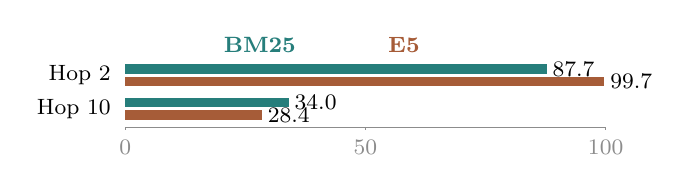
\begin{tikzpicture}[x=.061cm,y=.76cm,font=\footnotesize]
\draw[fill=tealchart,draw=none] (0,.98) rectangle (87.7,1.14);
\draw[fill=rustchart,draw=none] (0,.77) rectangle (99.7,.93);
\draw[fill=tealchart,draw=none] (0,.42) rectangle (34,.58);
\draw[fill=rustchart,draw=none] (0,.21) rectangle (28.4,.37);
\node[anchor=east] at (-1,.96) {Hop 2};
\node[anchor=east] at (-1,.39) {Hop 10};
\node[anchor=west,inner sep=2pt] at (87.7,1.06) {87.7};
\node[anchor=west,inner sep=2pt] at (99.7,.85) {99.7};
\node[anchor=west,inner sep=2pt] at (34,.50) {34.0};
\node[anchor=west,inner sep=2pt] at (28.4,.29) {28.4};
\draw[black!45] (0,.08)--(100,.08);
\foreach \x in {0,50,100} {\draw[black!45] (\x,.08)--(\x,.04) node[below] {\x};}
\node[text=tealchart,font=\footnotesize\bfseries] at (28,1.47) {BM25};
\node[text=rustchart,font=\footnotesize\bfseries] at (58,1.47) {E5};
\end{tikzpicture}
\end{center}
\smallcaption{Figure 3}{Gold-fact recall@20 (\%) at the shortest and longest hops. Data: \repo{results/t4/summary_retrieval.md}{retrieval-only audit}; all-gold recall is a separate metric.}

The S4 laptop probe used Qwen2.5-0.5B, 300 facts and five adapters. On the stronger training preset, HybridMem reached 38/60 seen and 36/60 paraphrased questions by a lenient contains scorer, versus 41/60 and 43/60 with plain retrieval. The task and model differ materially from the 7B multi-hop study. The probe verifies that the pipeline runs, not whether the paper's effect reproduces at scale.

\begin{center}
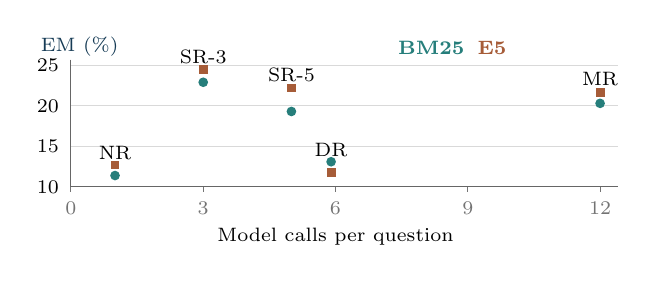
\begin{tikzpicture}[x=.56cm,y=.103cm,font=\footnotesize]
\foreach \y in {10,15,20,25} {
 \draw[black!15] (0,\y)--(12.4,\y);
 \node[anchor=east,font=\scriptsize] at (-.05,\y) {\y};
}
\draw[black!60] (0,25.7)--(0,10)--(12.4,10);
\foreach \x in {0,3,6,9,12} {
 \draw[black!55] (\x,10)--(\x,9.4) node[below,font=\scriptsize] {\x};
}
\node[anchor=east,font=\scriptsize,text=inkblue] at (1.3,27.3) {EM (\%)};
\node[font=\scriptsize] at (6,3.9) {Model calls per question};
\foreach \x/\a/\b in {1/11.4/12.7,3/22.9/24.5,5/19.3/22.2,5.9/13.1/11.8,12/20.3/21.6} {
 \fill[tealchart] (\x,\a) circle [radius=1.75pt];
 \fill[rustchart] ([xshift=-1.6pt,yshift=-1.6pt]\x,\b) rectangle ([xshift=1.6pt,yshift=1.6pt]\x,\b);
}
\foreach \x/\y/\n in {1/14.2/NR,3/26/SR-3,5/23.8/SR-5,5.9/14.6/DR,12/23.3/MR}
 \node[font=\scriptsize] at (\x,\y) {\n};
\node[text=tealchart,anchor=west,font=\scriptsize\bfseries] at (7.2,27.2) {BM25};
\node[text=rustchart,anchor=west,font=\scriptsize\bfseries] at (9,27.2) {E5};
\end{tikzpicture}
\end{center}
\smallcaption{Figure 4}{Observed cost and accuracy for Table 1 configurations. More calls did not guarantee better exact match. Call counts do not directly measure latency or token use.}

\clearpage
\section{Independent Discussion and Analysis}
\emphlabel{Numeric overlap is a shortcut risk, not proof of leakage.} Our \repo{results/probes/leak_check.md}{rule-based audit} flags questions that repeat a number from their gold evidence: 53\% overall and 82\% at hop 10. On S1, no-memory EM is 6.5\% on flagged questions versus 1.4\% on unflagged questions. That association is consistent with some questions permitting arithmetic from the question alone. An incidental date or number can also trigger the flag, and question difficulty may differ between groups. We therefore report both the full result and the unflagged subset instead of declaring all flagged items invalid.

\emphlabel{Upstream code and implementation limits.} We pinned the authors' released code to \href{https://github.com/nuster1128/MPR/tree/a24953c}{\texttt{a24953c}}. The \repo{docs/upstream-notes.md}{implementation audit} records missing official scoring code, an adapter-loading issue in BlockSFT, and an inefficient SFT padding path. Our evaluation uses a separate scorer and distinct adapter names, and the laptop runner pads batches dynamically. These changes let our experiments run and make comparisons within our study interpretable; they do not show that those issues affected the authors' published runs.

\emphlabel{What does not follow from this evidence.} We did not reproduce 7B multi-adapter training, trained MaskSFT, or TreeRAG/GraphRAG indexing. The matched sample uses a single seed. SR-5 changes prompt structure and number of calls; MR samples candidate branches while DR is greedy. DR begins without retrieved evidence and its Merge recall is lower than NR's; that identifies a candidate failure point, not a causal explanation. Controlled next tests are retrieval-aware versus blind decomposition, budget-matched fixed versus refreshed SR context, and reruns on independent samples and model revisions.


\noindent\cbox{\textbf{Article studied.} Zeyu Zhang, Yang Zhang, Haoran Tan, Rui Li, and Xu Chen. 2026. Explicit v.s. Implicit Memory: Exploring Multi-hop Complex Reasoning Over Personalized Information. In \emph{Proceedings of the 32nd ACM \mbox{SIGKDD} Conference on Knowledge Discovery and Data Mining V.1} (KDD '26), 1964--1974. \href{https://doi.org/10.1145/3770854.3780184}{DOI: 10.1145/3770854.3780184}. Our figure and table references use \href{https://arxiv.org/html/2508.13250v1}{arXiv:2508.13250v1}.}

\newpage
\section{Conclusion and Member Task Assignment}
\subsection{Conclusion}
Our independent study supports a limited but useful finding: answer accuracy is sensitive to reasoning structure, and does not reliably improve just because the system retrieves more evidence. SR and MR outperform one-call reasoning on the matched slice; DR's modest paper advantage over NR is not detectable in our runs. Short sequential chains offer a practical starting point because longer or branching methods did not clearly improve accuracy enough to justify the additional calls here. This is a recommendation to benchmark a baseline, not a claim that all deployed agents should use exactly three steps.

The fixed-evidence comparison makes the interpretation sharper: a major improvement occurs even when retrieval cannot improve. Conversely, raising recall through larger $k$ does not deliver detectable answer gains in our NR sweep. We would therefore measure evidence recall, answer quality and latency separately before choosing a retriever, step budget or adapter method. HybridMem should be tested where the benchmark and compute budget can distinguish a genuine benefit from configuration noise.

\subsection{Member tasks}
Nguyễn Xuân Phi was the primary contributor. Blank entries are to be completed by each member with their own contributions.

\begingroup\localtable
\noindent\begin{tabularx}{\columnwidth}{@{}>{\raggedright\arraybackslash}p{.34\columnwidth}>{\raggedright\arraybackslash}X@{}}
\toprule
\textbf{Member} & \textbf{Contribution} \\
\midrule
\vn{Nguyễn Xuân Phi} & Primary contributor: led the study and reproduction and synthesized the report and presentation. \\
\vn{Lê Hải Phong} &  \\
\vn{Trần Nguyên Phong} &  \\
\vn{Phan Văn Phú} &  \\
\bottomrule
\end{tabularx}
\endgroup

\smallskip
\noindent{\small\textbf{Evidence and reproducibility.} \repo{docs/reproduction-status.md}{Run ledger}, \repo{results/t4/summary_s2_vs_s1.md}{paired controls}, \repo{results/t4/summary_s3_topk_sweep.md}{top-$k$ sweep}, \repo{results/t4/summary_s3_steps_sweep.md}{step sweep}, \repo{results/t4/s5_mr/summary_mr.md}{MR traces}, \repo{results/t4/s6_dr/summary_dr.md}{DR comparison}, and \repo{results/laptop/sft/summary.md}{laptop results}. Links point to the team's repository and may need GitHub access.}
\end{document}
